% vim: set tw=78 softtabstop=4 shiftwidth=4 aw:
\documentclass{beamer}

\usepackage[utf8x]{inputenc} % diacritice
\usepackage[romanian]{babel}
\usepackage{color}			 % highlight
\usepackage{alltt}			 % highlight
\usepackage{hyperref}        % folositi \url{http://...}
\mode<presentation>
\usetheme{CDL}

\title[CSpay]{CSpay Standalone Version}
\subtitle{Proiect CDL}
\institute[ROSEdu]{ROSEdu}
\author[Răzvan Deaconescu]{Răzvan Deaconescu \\ \texttt{razvan@rosedu.org}}
\date{27 februarie 2010}

\begin{document}

\setbeamertemplate{frametitle continuation}[from second]
\setbeamertemplate{footline}[frame number]

\frame{\titlepage}

\section{CSpay Standalone Version}

\begin{frame}{What is this CSpay you speak of?}
    \begin{itemize}
	\pause \item Proiect de ``moravuri ușoare''
	\pause \item A fost ``atins'' de mai multe persoane
	    \begin{itemize}
		\pause \item Răzvan Deaconescu, Vlad Dogaru, Alex Eftimie, Mihai
Dumitrache, Andrei Buhaiu, Roxana Murăruș, Lucian Cojocar
		\pause \item Lucian Cojocar, Eduard Tuțescu, Alexandra Gherghina,
Paul Poida
		\pause \item Răzvan Deaconescu, Daniel Urdă, Grigore Lupescu
	    \end{itemize}
	\pause \item Continuous, progressive, chaotic development
	    \begin{itemize}
		\pause \item First make it work, then make it work!
	    \end{itemize}
	\pause \item Automatizarea unui proces birocratic financiar în facultate
	    \begin{itemize}
		\pause \item Nu sunt bani mulți. Nu vă gândiți la prostii! :-P
	    \end{itemize}
    \end{itemize}
\end{frame}

\begin{frame}{De ce aș contribui?}
    \begin{itemize}
	\pause \item It can't get no worse!
	\pause \item Multe zone de îmbunătățit
	\pause \item You can start small (bug fixing, code beautification)
	\pause \item Python
	\pause \item Feedback rapid -- vezi cum funcționează
	\pause \item Lucru cu documente, baze de date, date calendaristice, structuri
de date
    \end{itemize}
\end{frame}

\begin{frame}{Arhitectură}
    \begin{itemize}
	\pause \item \url{http://dev.rosedu.org/cspay}
	\pause \item \url{http://lists.rosedu.org/listinfo/cspay-dev}
    \end{itemize}
    \begin{figure}
	\pause 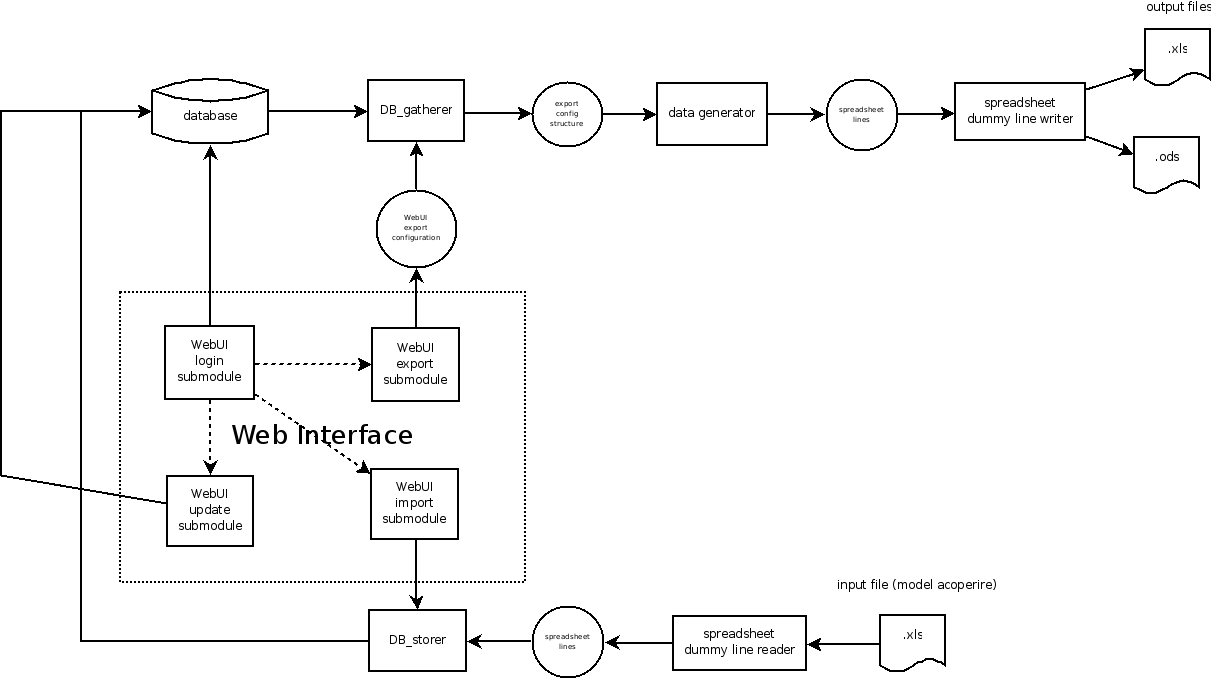
\includegraphics[scale=0.25]{img/cspay-architecture.png}
    \end{figure}
\end{frame}

\begin{frame}{Interfață}
    \begin{itemize}
	\pause \item \url{http://www.rosedu.org/~cspay/2009}
    \end{itemize}
    \begin{figure}
	\pause 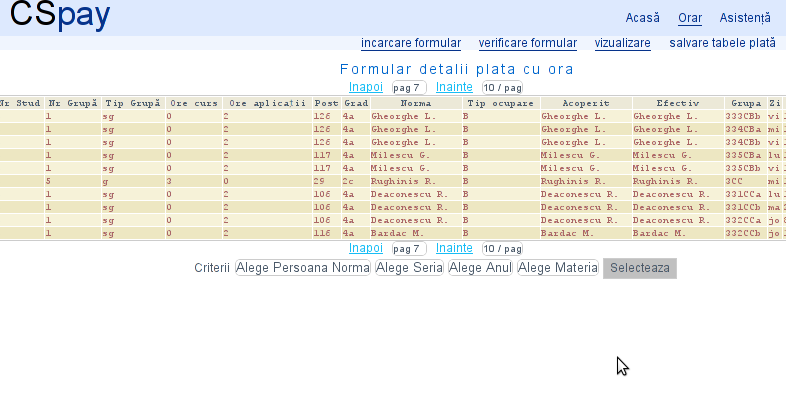
\includegraphics[scale=0.40]{img/cspay-interface.png}
    \end{figure}
\end{frame}

\begin{frame}{Cuvinte cheie \& întrebări}
    \begin{columns}
	\begin{column}[l]{0.5\textwidth}
	    \begin{itemize}
		\item CSpay
		\item standalone
		\item documente spredsheet
		\item baze de date
		\item SQlite
		\item Python
	    \end{itemize}
	\end{column}
	\begin{column}[c]{0.5\textwidth}
	    \begin{figure}
		\pause 
\includegraphics[scale=0.15]{img/question-mark.jpg}
	    \end{figure}
	\end{column}
    \end{columns}
\end{frame}

\end{document}
